\documentclass[12pt,a4paper]{book}
\newcommand{\niveau}{5\textsuperscript{e}}
\input{../../commun/preambule_commun}

\title{Cours de Mathématiques — Classe de 5\textsuperscript{e}\\[0.4em]\large Année scolaire 2025–2026}
\author{Abdoullatuf Maoulida}
%\date{\today}

\begin{document}
\maketitle
\tableofcontents
\cleardoublepage

%\part{Nombres et calculs}
\input{chapitres/seq_01} % Enchaînement d'opérations
% Sequence 2 : Symetrie centrale (5e)
\setseqtitle{Sym\'etrie centrale}
\chapter{Sym\'etrie centrale}

\begin{objectifsbox}
\textbf{Objectifs d'apprentissage.} À l'issue de la séquence, l'élève sera capable de :
\begin{itemize}
  \item Reconnaître et construire l'image d'une figure par symétrie centrale (centre donné)
  \item Utiliser les propriétés de conservation de la symétrie centrale
  \item Distinguer symétrie axiale et symétrie centrale
  \item Résoudre des problèmes géométriques en mobilisant la symétrie centrale
\end{itemize}
\end{objectifsbox}

\section{Rappel : symétrie axiale}

\begin{proprietebox}[Symétrie axiale]
La sym\'etrie axiale par rapport à une droite $d$ transforme tout point $M$ en un point $M'$ tel que $d$ est la médiatrice du segment $[MM']$. Elle conserve les longueurs, les angles et les aires.
\end{proprietebox}

\begin{examplebox}[Illustration]
\begin{center}
\begin{tikzpicture}[scale=0.9]
  % Axe de symetrie d (vertical)
  \draw[blue!60, very thick, dashed] (0,-2) -- (0,2) node[above]{$d$};
  % Points A et A' symetriques par rapport a d
  \coordinate (A) at (-2,1.2);
  \coordinate (Aprime) at (2,1.2);
  \draw[fill=black] (A) circle (1.5pt) node[above left]{$A$};
  \draw[fill=black] (Aprime) circle (1.5pt) node[above right]{$A'$};
  % Perpendiculaires
  \draw[gray,code1] (A) -- (0,1.2);
  \draw[gray,code1] (Aprime) -- (0,1.2);
\end{tikzpicture}
\end{center}
\end{examplebox}

\section{Découverte : symétrie centrale}

% Activité: deux symétries axiales successives
\begin{activitybox}[Deux symétries axiales pour une centrale]
\textbf{Consigne.}
\begin{enumerate}
  \item On considère deux droites \textbf{perpendiculaires} $d_1$ et $d_2$ qui se coupent en $I$.
  \item Construire une petite figure $F_0$ (par exemple un triangle ou la lettre \og L \fg{}).
  \item Construire $F_1$, image de $F_0$ par la symétrie axiale d'axe $d_1$.
  \item Construire $F_2$, image de $F_1$ par la symétrie axiale d'axe $d_2$.
  \item Comment passer directement de $F_0$ à $F_2$ sans pliage ni étape intermédiaire ?
\end{enumerate}

\begin{center}
	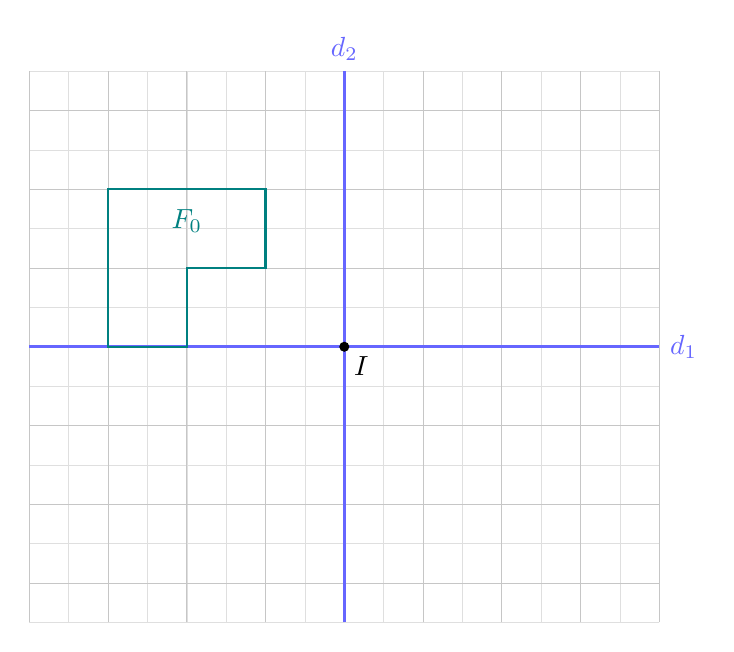
\begin{tikzpicture}[scale=1]
		% Grille (mineure 0.5, majeure 1)
		\draw[help lines, color=gray!25, step=0.5] (-4,-3.5) grid (4,3.5);
		\draw[help lines, color=gray!45, line width=0.25pt, step=1] (-4,-3.5) grid (4,3.5);
		
		% Axes perpendiculaires
		\coordinate (I) at (0,0);
		\draw[very thick, blue!60] (-4,0) -- (4,0) node[right]{$d_1$};
		\draw[very thick, blue!60] (0,-3.5) -- (0,3.5) node[above]{$d_2$};
		\draw[fill=black] (I) circle (1.6pt) node[below right]{$I$};
		
		% Figure F0 : lettre L, sommets sur la grille (entiers)
		\coordinate (P1) at (-3,2);
		\coordinate (P2) at (-1,2);
		\coordinate (P3) at (-1,1);
		\coordinate (P4) at (-2,1);
		\coordinate (P5) at (-2,0);
		\coordinate (P6) at (-3,0);
		\draw[thick, teal] (P1)--(P2)--(P3)--(P4)--(P5)--(P6)--cycle;
		\node[teal] at (-2,1.6) {$F_0$};
	\end{tikzpicture}
\end{center}

\trous{14cm}\\
\trous{14cm}\\
\trous{14cm}
\end{activitybox}


\begin{definitionbox}[Symétrie centrale]
	La \textbf{symétrie centrale} de centre $O$ est la transformation qui laisse $O$ invariant et qui transforme tout point $M$ en un point $M'$ tel que \textbf{$O$ est le milieu de $[MM']$}.
\end{definitionbox}

% L'ILLUSTRATION RESTE PARFAITE
\begin{examplebox}[Illustration]
	\begin{center}
		\begin{tikzpicture}[scale=1]
			\coordinate (O) at (0,0);
			\coordinate (M) at (2,1);
			\coordinate (M') at (-2,-1);
			\draw[fill=black] (O) circle (1.5pt) node[below right]{$O$};
			\draw[fill=black] (M) circle (1.5pt) node[above]{$M$};
			\draw[fill=black] (M') circle (1.5pt) node[below]{$M'$};
			\draw[gray] (M) -- (M');
			% Suggestion d'amélioration pour le placement du mot "milieu"
			\node[anchor=south west, xshift=1pt, yshift=1pt, inner sep=1pt, fill=white] at (O) {\small milieu};
		\end{tikzpicture}
	\end{center}
\end{examplebox}

\section{Figures symétriques par rapport à un point}
\begin{definitionbox}
Deux figures sont symétriques par rapport à un point $O$ lorsqu'elles \\
se superposent en \trous{10cm}\\
autour de ce point.
On dit que $O$ est le centre de la symétrie.
\end{definitionbox}

\begin{examplebox}
	\begin{center}
		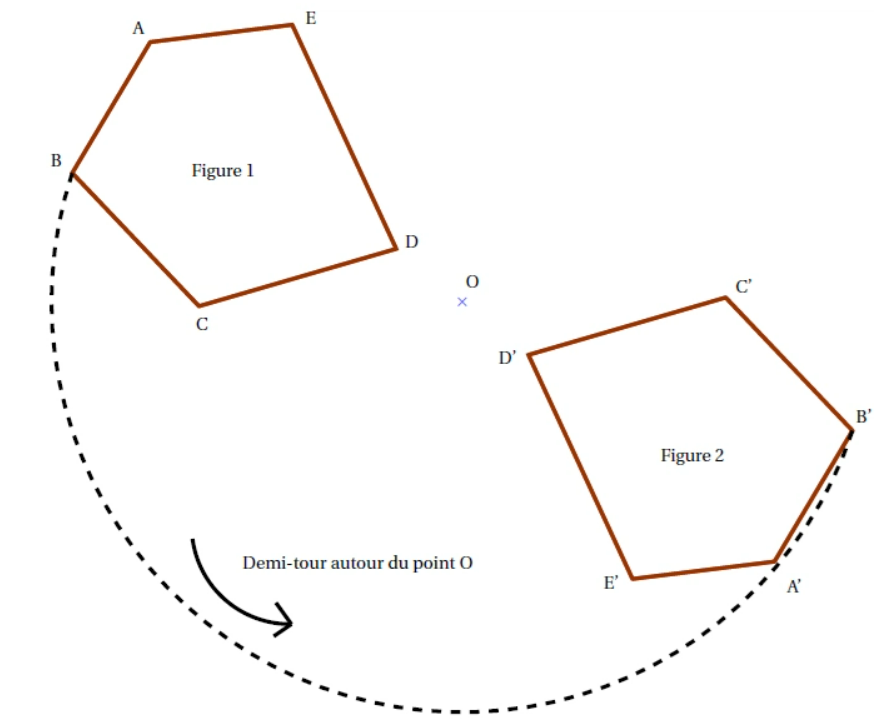
\includegraphics[width=0.6\linewidth]{../../assets/images/5e/seq_02/figures_symetriques}
	\end{center}
	
\end{examplebox}	

\section{Symétrique d'un point par rapport à un point}

\begin{definitionbox}
	Le symétrique d’un point $M$ par rapport à un point $O$ est le point $M'$ tel que le point $O$ est le milieu du segment $[MM']$.
\end{definitionbox}

\begin{examplebox}
	Placer le symétrique $A'$ du point $A$ par rapport au point $O$ en utilisant le quadrillage.
	\begin{center}
		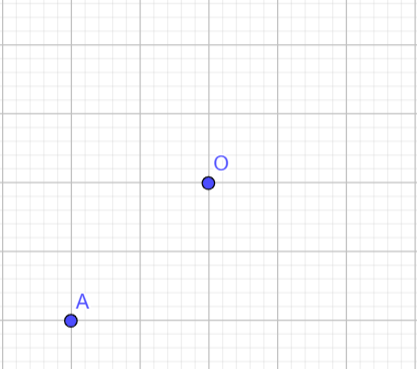
\includegraphics[width=0.7\linewidth]{../../assets/images/5e/seq_02/exemple_image_point_construction}
	\end{center}
	

\end{examplebox}	

\section{Constructions}

\subsection{Image d'un point}
\begin{methodebox}[Point à point]
Pour construire l'image $A'$ d'un point $A$ par la symétrie centrale de centre $O$ :
\begin{enumerate}
  \item Tracer la demi-droite $[AO)$.
  \item Reporter $OA$ de l'autre côté de $O$ pour obtenir le point $A'$ avec $OA'=OA$ (à la règle et au compas).
  \item Vérifier que $O$ est le milieu de $[AA']$.
\end{enumerate}


\begin{center}
	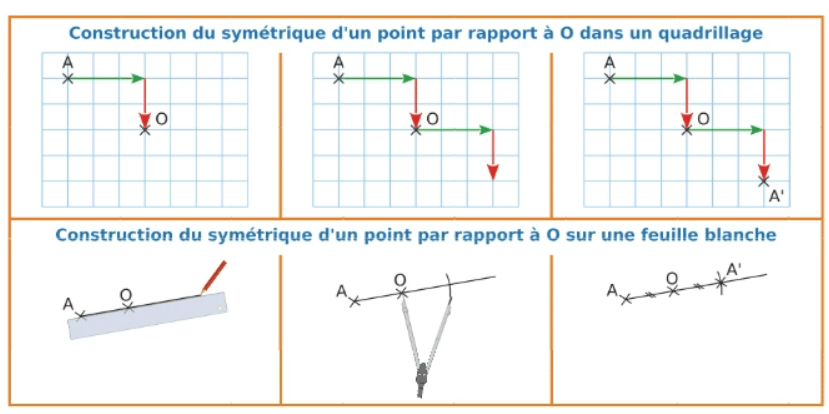
\includegraphics[width=1\linewidth]{../../assets/images/5e/seq_02/methode_construction_point_par_symetrie_centrale}
\end{center}

\end{methodebox}



\subsection{Image d'une figure}
\begin{methodebox}[Segment, droite, triangle]
\begin{itemize}
  \item \textbf{Segment $[AB]$} \;$\to$\; \textit{$[A'B']$ parall\`ele et de m\^eme longueur}.
  \item \textbf{Droite $(d)$} \;$\to$\; \textit{droite $d'$ parallèle à $(d)$} (si $(d)$ passe par $O$, elle est invariante).
  \item \textbf{Triangle $ABC$} \;$\to$\; \textit{triangle $A'B'C'$ superposable par demi-tour (aires et angles conserv\'es)}.
\end{itemize}
\end{methodebox}

\begin{examplebox}[Construction par symétrie centrale]
	Construire l’image du triangle $ABC$ par la symétrie centrale de centre $O$. Laisser visibles les traits de construction et nommer $A'$, $B'$, $C'$.
	
	\begin{center}
		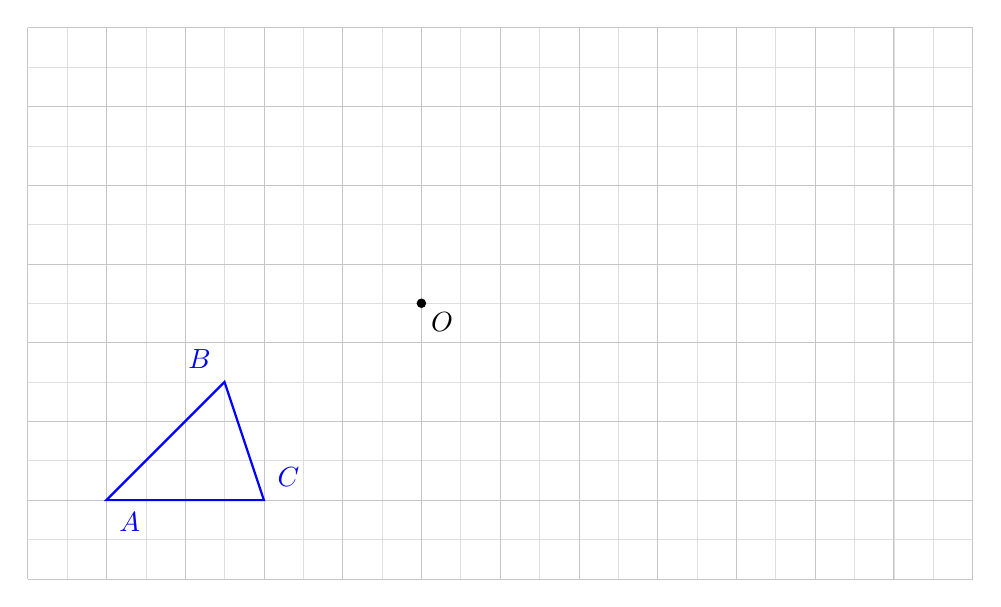
\begin{tikzpicture}[x=1cm,y=1cm]
			% Zone de dessin
			\useasboundingbox (0,0) rectangle (12,7);
			
			% Quadrillage (mineur 0.5, majeur 1)
			\draw[help lines, color=gray!25, step=0.5] (0,0) grid (12,7);
			\draw[help lines, color=gray!45, line width=0.25pt, step=1] (0,0) grid (12,7);
			
			% Centre O (au centre)
			\coordinate (O) at (5,3.5);
			\draw[fill=black] (O) circle (1.5pt);
			\node[below right] at (O) {$O$};
			
			% Triangle ABC en bas à gauche (sommets sur la grille)
			\coordinate (A) at (1,1);
			\coordinate (B) at (2.5,2.5);
			\coordinate (C) at (3,1);
			\draw[thick, blue] (A)--(B)--(C)--cycle;
			
			% Étiquettes bien placées
			\node[below right, xshift=0.4mm, yshift=-0.4mm, blue] at (A) {$A$};
			\node[above left, xshift=-0.5mm, yshift=0.5mm, blue] at (B) {$B$};
			\node[above right, xshift=0.5mm, yshift=0.5mm, blue] at (C) {$C$};
		\end{tikzpicture}
	\end{center}
\end{examplebox}

\section{Propriétés}

\begin{proprietebox}[Conservations]
La sym\'etrie centrale (centre $O$) :
\begin{itemize}
  \item conserve les longueurs, les angles et les aires ;
  \item envoie une droite ne passant pas par $O$ sur une droite \textbf{parall\`ele} ;
  \item laisse inchang\'ee toute droite passant par $O$ ;
  \item transforme un cercle en un cercle de m\^eme rayon ;
  \item est \textbf{\'equivalente au demi-tour} (rotation d'angle $180^{\circ}$) de centre $O$.
\end{itemize}
\end{proprietebox}

\begin{remarkbox}
Une figure qui admet un centre de sym\'etrie est dite \textbf{centrosym\'etrique} (ex. : parall\'elogramme, rectangle, losange, cercle).
\end{remarkbox}

\section{Centre de symétrie d'une figure}

\begin{definitionbox}[Centre de symétrie]
Une figure $\mathcal F$ \textbf{admet un centre de symétrie} s'il existe un point $O$ tel que la symétrie centrale de centre $O$ laisse $\mathcal F$ \textbf{inchangée} (chaque point de $\mathcal F$ a son image encore dans $\mathcal F$). On dit alors que $O$ est \textbf{centre de symétrie} de $\mathcal F$.
\end{definitionbox}

\begin{examplebox}[Exemples et contre-exemples]
\begin{itemize}
  \item Segment $[AB]$ : centre $I$, \textbf{milieu} de $[AB]$.
  \item Cercle ou disque : \textbf{son centre}.
  \item Parallélogramme, rectangle, losange : \textbf{intersection des diagonales}.
  \item Triangle quelconque, lettre \og L\fg{} : \textbf{pas} de centre de symétrie.
\end{itemize}

\begin{center}
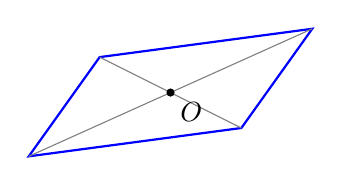
\begin{tikzpicture}[scale=0.9]
  % Parallélogramme avec centre
  \coordinate (A) at (0,0);
  \coordinate (B) at (3,0.4);
  \coordinate (C) at (4,1.8);
  \coordinate (D) at (1,1.4);
  \draw[thick,blue] (A)--(B)--(C)--(D)--cycle;
  \draw[gray] (A)--(C) (B)--(D);
  \path (A)--(C) coordinate[pos=0.5] (O);
  \draw[fill=black] (O) circle (1.4pt) node[below right]{$O$};
\end{tikzpicture}
\end{center}
\end{examplebox}

\begin{methodebox}[Comment le trouver ?]
\begin{itemize}
  \item \textbf{Segment} : prendre le \textbf{milieu}.
  \item \textbf{Parallélogramme/rectangle/losange} : tracer les \textbf{deux diagonales} et prendre leur \textbf{intersection}.
  \item \textbf{Cercle/disque} : le \textbf{centre} du cercle.
  \item \textbf{Polygone régulier à nombre pair de côtés} : centre du polygone. À nombre impair : \textbf{pas} de centre de symétrie.
\end{itemize}
\end{methodebox}

%\begin{proprietebox}[Unicité et cas particuliers]
%Pour une figure \textbf{bornée} (segment, polygone, disque, etc.), s'il existe, le centre de symétrie est en général \textbf{unique}. Une \textbf{droite} admet au contraire une infinité de centres : \textbf{tous ses points}.
%\end{proprietebox}

\clearpage
\section{Comparaison : axiale vs centrale}

\begin{methodebox}[Comment les distinguer ?]
\begin{itemize}
  \item \textbf{Axiale} : on cherche une \textit{droite} qui partage la figure en deux parties superposables.
  \item \textbf{Centrale} : on cherche un \textit{point $O$} tel que toute droite passant par $O$ coupe la figure en deux points sym\'etriques (milieu en $O$).
\end{itemize}
\end{methodebox}

\section{Exercices d'application}

\begin{exercisebox}
\textbf{Exercice 1 (construction)}. On donne un point $O$ et des points $A$, $B$, $C$.
\begin{enumerate}
  \item Construire $A'$, $B'$, $C'$ images de $A$, $B$, $C$ par la sym\'etrie centrale de centre $O$.
  \item Que peut-on dire des segments $[AB]$ et $[A'B']$ ? des angles $\widehat{ABC}$ et $\widehat{A'B'C'}$ ?
\end{enumerate}
\end{exercisebox}

\begin{exercisebox}
\textbf{Exercice 2 (triangle)}. Construire l'image du triangle $ABC$ par la sym\'etrie centrale de centre $O$. Tracer ensuite les droites $(AA')$, $(BB')$, $(CC')$ : que remarquez-vous ?
\end{exercisebox}

\begin{exercisebox}
\textbf{Exercice 3 (droites et cercles)}. Soit une droite $(d)$ qui ne passe pas par $O$ et un cercle $\mathcal C$ de centre $A$ passant par $B$.
\begin{enumerate}
  \item Construire l'image $(d')$ de $(d)$.
  \item Construire l'image $\mathcal C'$ de $\mathcal C$ et pr\'eciser son centre et son rayon.
\end{enumerate}
\end{exercisebox}

\begin{exercisebox}
\textbf{Exercice 4 (vrai/faux)}. Dire si les affirmations sont vraies ou fausses et justifier.
\begin{enumerate}
  \item Par sym\'etrie centrale, un rectangle devient un parall\'elogramme.
  \item L'image d'une droite par une sym\'etrie centrale est toujours la même droite.
  \item Si $ABCD$ est un parall\'elogramme, alors $O$, intersection des diagonales, est un centre de sym\'etrie.
\end{enumerate}
\end{exercisebox}

\begin{quizbox}
\textbf{Auto-\'evaluation rapide}
\begin{enumerate}[label=\arabic*)]
  \item Donner la d\'efinition de l'image d'un point par sym\'etrie centrale.
  \item Citer deux propri\'et\'es conserv\'ees par la sym\'etrie centrale.
  \item Expliquer comment distinguer visuellement une symétrie axiale d'une symétrie centrale.
\end{enumerate}
\end{quizbox}

\clearpage
\section*{Corrigés des exercices d'application}

\begin{solutionbox}
	\textbf{Exercice 1 — Correction}
	\begin{enumerate}
		\item Pour construire l'image de chaque point ($A$, $B$ ou $C$) :
		\begin{itemize}
			\item Tracer la droite passant par $O$ et le point (par exemple $A$).
			\item Placer le point image $A'$ de l'autre côté de $O$, à la même distance : $OA' = OA$.
			\item Ainsi, $O$ est le milieu du segment $[AA']$.
			\item Faire de même pour $B$ et $C$.
		\end{itemize}

		\begin{center}
		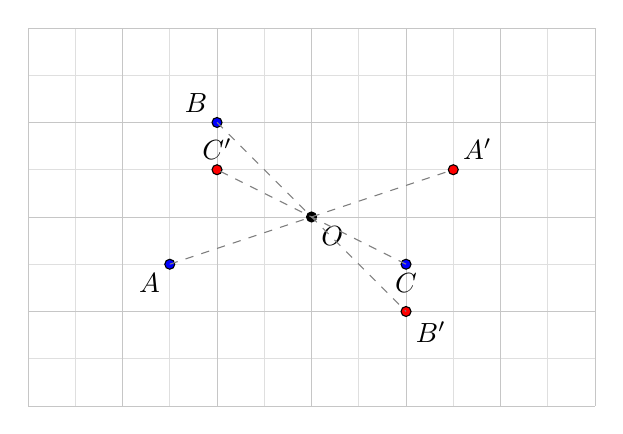
\begin{tikzpicture}[scale=1.2]
			% Grille
			\draw[help lines, color=gray!25, step=0.5] (-1,-1) grid (5,3);
			\draw[help lines, color=gray!45, line width=0.25pt, step=1] (-1,-1) grid (5,3);

			% Centre O
			\coordinate (O) at (2,1);
			\draw[fill=black] (O) circle (1.5pt) node[below right]{$O$};

			% Points A, B, C
			\coordinate (A) at (0.5,0.5);
			\coordinate (B) at (1,2);
			\coordinate (C) at (3,0.5);
			\draw[fill=blue] (A) circle (1.5pt) node[below left]{$A$};
			\draw[fill=blue] (B) circle (1.5pt) node[above left]{$B$};
			\draw[fill=blue] (C) circle (1.5pt) node[below]{$C$};

			% Images A', B', C'
			\coordinate (A') at (3.5,1.5);
			\coordinate (B') at (3,0);
			\coordinate (C') at (1,1.5);
			\draw[fill=red] (A') circle (1.5pt) node[above right]{$A'$};
			\draw[fill=red] (B') circle (1.5pt) node[below right]{$B'$};
			\draw[fill=red] (C') circle (1.5pt) node[above]{$C'$};

			% Droites de construction
			\draw[gray, dashed] (A) -- (A');
			\draw[gray, dashed] (B) -- (B');
			\draw[gray, dashed] (C) -- (C');
		\end{tikzpicture}
		\end{center}

		\item Les segments $[AB]$ et $[A'B']$ ont la même longueur et sont parallèles. De même, les angles $\widehat{ABC}$ et $\widehat{A'B'C'}$ ont la même mesure (la symétrie centrale conserve les longueurs et les angles).
	\end{enumerate}
\end{solutionbox}

\begin{solutionbox}
	\textbf{Exercice 2 — Correction}

	On construit l'image du triangle $ABC$ en trouvant les points $A'$, $B'$, $C'$ images de $A$, $B$, $C$ par la symétrie centrale de centre $O$.

	\begin{center}
	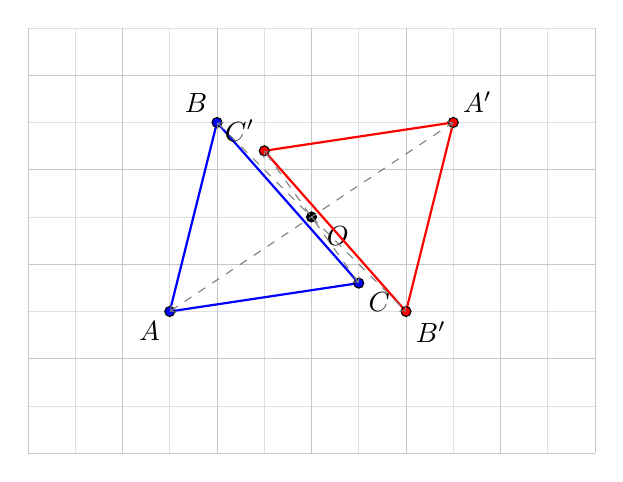
\begin{tikzpicture}[scale=1.2]
		% Grille
		\draw[help lines, color=gray!25, step=0.5] (-1,-1) grid (5,3.5);
		\draw[help lines, color=gray!45, line width=0.25pt, step=1] (-1,-1) grid (5,3.5);

		% Centre O
		\coordinate (O) at (2,1.5);
		\draw[fill=black] (O) circle (1.5pt) node[below right, xshift=2pt]{$O$};

		% Triangle ABC
		\coordinate (A) at (0.5,0.5);
		\coordinate (B) at (1,2.5);
		\coordinate (C) at (2.5,0.8);
		\draw[thick, blue] (A) -- (B) -- (C) -- cycle;
		\draw[fill=blue] (A) circle (1.5pt) node[below left]{$A$};
		\draw[fill=blue] (B) circle (1.5pt) node[above left]{$B$};
		\draw[fill=blue] (C) circle (1.5pt) node[below right]{$C$};

		% Triangle A'B'C'
		\coordinate (A') at (3.5,2.5);
		\coordinate (B') at (3,0.5);
		\coordinate (C') at (1.5,2.2);
		\draw[thick, red] (A') -- (B') -- (C') -- cycle;
		\draw[fill=red] (A') circle (1.5pt) node[above right]{$A'$};
		\draw[fill=red] (B') circle (1.5pt) node[below right]{$B'$};
		\draw[fill=red] (C') circle (1.5pt) node[above left]{$C'$};

		% Droites passant par O
		\draw[gray, dashed, <->] (A) -- (A');
		\draw[gray, dashed, <->] (B) -- (B');
		\draw[gray, dashed, <->] (C) -- (C');
	\end{tikzpicture}
	\end{center}

	\textbf{Observation :} Les trois droites $(AA')$, $(BB')$ et $(CC')$ passent toutes par le point $O$. En effet, $O$ est le milieu de chaque segment $[AA']$, $[BB']$ et $[CC']$, donc toutes ces droites se coupent en $O$.
\end{solutionbox}

\begin{solutionbox}
	\textbf{Exercice 3 — Correction}
	\begin{enumerate}
		\item Pour construire l'image $(d')$ de la droite $(d)$ :
		\begin{itemize}
			\item Choisir deux points sur $(d)$, par exemple $P$ et $Q$.
			\item Construire leurs images $P'$ et $Q'$ par la symétrie de centre $O$.
			\item La droite $(d')$ passe par $P'$ et $Q'$.
			\item Puisque $(d)$ ne passe pas par $O$, la droite $(d')$ est parallèle à $(d)$.
		\end{itemize}

		\begin{center}
		\begin{tikzpicture}[scale=1.1]
			% Grille
			\draw[help lines, color=gray!25, step=0.5] (-0.5,-0.5) grid (6,3.5);
			\draw[help lines, color=gray!45, line width=0.25pt, step=1] (-0.5,-0.5) grid (6,3.5);

			% Centre O
			\coordinate (O) at (2.5,1.5);
			\draw[fill=black] (O) circle (1.5pt) node[below right]{$O$};

			% Droite (d) et points P, Q
			\coordinate (P) at (0.5,0.8);
			\coordinate (Q) at (2,0.3);
			\draw[thick, blue] (0,1) -- (3,0) node[right]{$(d)$};
			\draw[fill=blue] (P) circle (1.5pt) node[above left]{$P$};
			\draw[fill=blue] (Q) circle (1.5pt) node[above right]{$Q$};

			% Images P' et Q' par symétrie de centre O
			\coordinate (P') at (4.5,2.2);
			\coordinate (Q') at (3,2.7);
			\draw[fill=red] (P') circle (1.5pt) node[below right]{$P'$};
			\draw[fill=red] (Q') circle (1.5pt) node[below left]{$Q'$};

			% Droite (d') passant par P' et Q'
			\draw[thick, red] ($(P')!-0.3!(Q')$) -- ($(Q')!-0.3!(P')$) node[right]{$(d')$};

			% Droites de construction
			\draw[gray, dashed] (P) -- (P');
			\draw[gray, dashed] (Q) -- (Q');
		\end{tikzpicture}
		\end{center}

		\item Pour construire l'image $\mathcal C'$ du cercle $\mathcal C$ :
		\begin{itemize}
			\item Trouver l'image $A'$ du centre $A$ par la symétrie de centre $O$.
			\item Le cercle $\mathcal C'$ a pour centre $A'$.
			\item Son rayon est le même que celui de $\mathcal C$, c'est-à-dire $AB$ (ou $A'B' = AB$).
		\end{itemize}

		\begin{center}
		\begin{tikzpicture}[scale=1.1]
			% Grille
			\draw[help lines, color=gray!25, step=0.5] (-0.5,-0.5) grid (6,3.5);
			\draw[help lines, color=gray!45, line width=0.25pt, step=1] (-0.5,-0.5) grid (6,3.5);

			% Centre O
			\coordinate (O) at (3,1.5);
			\draw[fill=black] (O) circle (1.5pt) node[below right]{$O$};

			% Cercle C
			\coordinate (A) at (1.5,1);
			\draw[thick, blue] (A) circle (0.7cm);
			\draw[fill=blue] (A) circle (1.5pt) node[below left]{$A$};
			% B sur le cercle : angle 45 degrés, rayon 0.7cm
			\coordinate (B) at ($(A) + (45:0.7cm)$);
			\draw[fill=blue] (B) circle (1.5pt) node[above right]{$B$};
			\node[blue] at (1.5,0) {$\mathcal C$};

			% Cercle C' (image de C par symétrie de centre O)
			\coordinate (A') at (4.5,2);
			\draw[thick, red] (A') circle (0.7cm);
			\draw[fill=red] (A') circle (1.5pt) node[above right]{$A'$};
			% B' image de B par symétrie de centre O : B' = 2*O - B
			\coordinate (B') at ($(2*3,2*1.5) - (B)$);
			\draw[fill=red] (B') circle (1.5pt) node[below left]{$B'$};
			\node[red] at (4.5,3) {$\mathcal C'$};

			% Droites de construction
			\draw[gray, dashed] (A) -- (A');
			\draw[gray, dashed] (B) -- (B');
		\end{tikzpicture}
		\end{center}
	\end{enumerate}
\end{solutionbox}

\begin{solutionbox}
	\textbf{Exercice 4 — Correction}
	\begin{enumerate}
		\item \textbf{Vrai.} Un rectangle reste un rectangle par symétrie centrale (donc c'est aussi un parallélogramme).

		\item \textbf{Faux.} L'image d'une droite par symétrie centrale est la même droite seulement si la droite passe par le centre $O$. Sinon, l'image est une droite parallèle mais différente.

		\item \textbf{Vrai.} Dans un parallélogramme $ABCD$, le point $O$ (intersection des diagonales) est un centre de symétrie : il échange les sommets opposés ($A$ avec $C$, et $B$ avec $D$).

		\begin{center}
		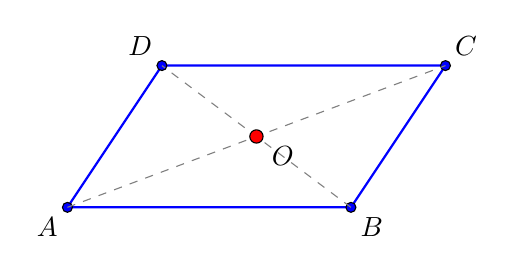
\begin{tikzpicture}[scale=1.2]
			% Parallélogramme ABCD
			\coordinate (A) at (0,0);
			\coordinate (B) at (3,0);
			\coordinate (C) at (4,1.5);
			\coordinate (D) at (1,1.5);
			\draw[thick, blue] (A) -- (B) -- (C) -- (D) -- cycle;
			\draw[fill=blue] (A) circle (1.5pt) node[below left]{$A$};
			\draw[fill=blue] (B) circle (1.5pt) node[below right]{$B$};
			\draw[fill=blue] (C) circle (1.5pt) node[above right]{$C$};
			\draw[fill=blue] (D) circle (1.5pt) node[above left]{$D$};

			% Diagonales
			\draw[gray, dashed] (A) -- (C);
			\draw[gray, dashed] (B) -- (D);

			% Centre O
			\coordinate (O) at (2,0.75);
			\draw[fill=red] (O) circle (2pt) node[below right, xshift=2pt]{$O$};
		\end{tikzpicture}
		\end{center}
	\end{enumerate}
\end{solutionbox}

\begin{solutionbox}
	\textbf{Auto-évaluation rapide — Corrigé}
	\begin{enumerate}[label=\arabic*)]
		\item L'image d'un point $M$ par la symétrie centrale de centre $O$ est le point $M'$ tel que $O$ soit le milieu du segment $[MM']$.
		\item Propriétés conservées : longueurs, mesures d'angles, alignement, parallélisme, aires.
		\item \textbf{Symétrie axiale :} on plie la figure le long d'une droite (l'axe). \textbf{Symétrie centrale :} on fait tourner la figure d'un demi-tour autour d'un point (le centre).
	\end{enumerate}
\end{solutionbox}

 % symétrie centrale
% Séquence 3 : Nombres en écriture fractionnaire (5e)
\setseqtitle{Nombres en écriture fractionnaire}
\chapter{Nombres en écriture fractionnaire}

\begin{objectifsbox}
	\textbf{Objectifs d'apprentissage.} À l'issue de la séquence, l'élève sera capable de :
	\begin{itemize}
		\item Comprendre les différentes interprétations d'une fraction
		\item Reconnaître et produire des fractions égales
		\item Simplifier une fraction par division
		\item Décomposer une fraction en somme d'un entier et d'une fraction inférieure à 1
		\item Comparer des fractions entre elles
		\item Encadrer une fraction par deux entiers consécutifs
	\end{itemize}
\end{objectifsbox}

\section{Différentes significations d'une fraction}

\subsection{Activité d'introduction}

\begin{activitybox}[Manipulation : Le chocolat partagé]
	\textbf{Matériel :} Feuilles de papier représentant des tablettes de chocolat.
	
	\textbf{Situation 1 :} On a 3 tablettes de chocolat à partager équitablement entre 4 personnes.
	\begin{enumerate}[label=\alph*)]
		\item Dessiner comment on pourrait découper les tablettes.
		\item Quelle quantité reçoit chaque personne ?
		\item Écrire cette quantité sous forme de fraction.
	\end{enumerate}
	
	\textbf{Situation 2 :} Maintenant, on a 1 tablette à partager entre 4 personnes.
	\begin{enumerate}[label=\alph*)]
		\item Quelle fraction de la tablette reçoit chaque personne ?
		\item Comparer les deux situations. Que remarque-t-on ?
	\end{enumerate}
	
	\trous{10cm}
\end{activitybox}

\begin{activitybox}[Manipulation : Le Partage Équitable des Bandes]
	\textbf{Objectif :} Découvrir la notion de fraction par la manipulation concrète.
	
	\textbf{Matériel nécessaire :}
	\begin{itemize}
		\item Une bande unité de 21 cm (papier coloré ou cartonné)
		\item Des bandes à mesurer : 10,5 cm ; 7 cm ; 15,75 cm ; 5,25 cm
		\item Des bandes blanches vierges pour reproduire
		\item Règle, ciseaux, crayon
	\end{itemize}
	
	\medskip
	
	\textbf{Phase 1 : Découverte (15 min)}
	
	\textbf{Consigne :} Votre professeur vous donne une bande unité et une bande à mesurer. Sans utiliser la règle, trouvez un moyen de fabriquer une bande exactement de la même longueur que la bande à mesurer en utilisant \textbf{uniquement} la bande unité.
	
	\textbf{Méthodes possibles :}
	\begin{itemize}
		\item Plier la bande unité en 2, 4 ou 8 parties égales
		\item Superposer et ajuster
		\item Reproduire en découpant des bandes blanches
	\end{itemize}
	
	\trous{10cm}
	
	\medskip
	
	\textbf{Phase 2 : Verbalisation (10 min)}
	
	Présenter votre méthode à la classe. Compléter les phrases suivantes :
	
	\begin{itemize}
		\item « J'ai plié ma bande unité en \trous{3cm} parties égales »
		\item « J'ai pris \trous{3cm} de ces parties »
		\item « Ma bande mesure \trous{5cm} de l'unité »
	\end{itemize}
	
	\medskip
	
	\textbf{Phase 3 : Symbolisation (10 min)}
	
	On note cette longueur avec une \textbf{fraction} :
	
	\begin{center}
		\begin{tikzpicture}[scale=0.25]
			\node at (0,0) {$\dfrac{\text{nombre de parts prises}}{\text{nombre de parts au total}}$};
		\end{tikzpicture}
	\end{center}
	
	\textbf{Exemples :}
	\begin{itemize}
		\item Bande de 10,5 cm = $\frac{1}{2}$ de l'unité (la moitié)
		\item Bande de 7 cm = $\frac{1}{3}$ de l'unité (un tiers)
		\item Bande de 15,75 cm = $\frac{3}{4}$ de l'unité (trois quarts)
	\end{itemize}
	
	\medskip
	
	\textbf{Phase 4 : Exploration (15 min)}
	
	Compléter le tableau suivant en mesurant et en exprimant chaque bande sous forme de fraction :
	
	\begin{center}
		\begin{tabular}{|c|c|c|}
			\hline
			\textbf{Bande} & \textbf{Longueur mesurée} & \textbf{Fraction de l'unité} \\
			\hline
			A & \trous{3cm} & \trous{3cm} \\
			\hline
			B & \trous{3cm} & \trous{3cm} \\
			\hline
			C & \trous{3cm} & \trous{3cm} \\
			\hline
		\end{tabular}
	\end{center}
	
	\medskip
	
	\textbf{Question :} Peut-on avoir une fraction supérieure à 1 ? Si oui, donner un exemple.
	
	\trous{10cm}
\end{activitybox}

\subsection{Vocabulaire et notation}

\begin{definitionbox}[Écriture fractionnaire]
	\begin{minipage}[t]{0.62\textwidth}
		Une \textbf{fraction} est un nombre qui s'écrit sous la forme $\dfrac{a}{b}$ où $a$ et $b$ sont deux nombres entiers avec $b \neq 0$.
		
		\begin{itemize}
			\item Le nombre du haut, $a$, s'appelle le \textbf{numérateur}.
			\item Le nombre du bas, $b$, s'appelle le \textbf{dénominateur}.
			\item Le trait de fraction signifie « divisé par ».
		\end{itemize}
	\end{minipage}%
	\hfill
	\begin{minipage}[t]{0.33\textwidth}
		\centering
		\vspace{0.5cm}
		\Huge\tikzmarknode{fracA}{$\dfrac{\tikzmarknode{numA}{a}}{\tikzmarknode{denA}{b}}$}
		\begin{tikzpicture}[overlay, remember picture]
			\draw[->, thick, mainRed] ([yshift=8mm]numA.north) node[above, black] {\normalsize numérateur} -- (numA.north);
			\draw[->, thick, mainBlue] ([yshift=-8mm]denA.south) node[below, black] {\normalsize dénominateur} -- (denA.south);
		\end{tikzpicture}
	\end{minipage}
\end{definitionbox}


\begin{remarkbox}
	\begin{itemize}
		\item On lit $\frac{3}{4}$ : « trois quarts » ou « trois sur quatre ».
		\item Une fraction représente le \textbf{quotient} : $\frac{a}{b} = a \div b$.
		\item Le dénominateur ne peut \textbf{jamais} être égal à zéro (on ne peut pas diviser par zéro).
	\end{itemize}
\end{remarkbox}

\begin{examplebox}
	\textbf{Interprétations de $\frac{5}{2}$ :}
	\begin{itemize}
		\item \textbf{Partage :} On prend 5 parts d'un objet découpé en 2 parts égales.
		\item \textbf{Quotient :} $\frac{5}{2} = 5 \div 2 = 2,5$
		\item \textbf{Fraction supérieure à 1 :} $\frac{5}{2} = \frac{..... + .....}{.....} = \frac{ .....}{.....} +\frac{ .....}{.....} = .... + \frac{.....}{....}$
	\end{itemize}
	
	\textbf{Représentations visuelles de $\frac{3}{4}$ :}
	
\begin{center}
	\begin{tikzpicture}[scale=0.8]
		% Disque (camembert) - Inchangé
		\draw[thick] (0,0) circle (1);
		\fill[mainGreen!40] (0,0) -- (1,0) arc (0:270:1) -- cycle;
		\draw[thick] (0,0) -- (1,0);
		\draw[thick] (0,0) -- (0,1);
		\draw[thick] (0,0) -- (-1,0);
		\draw[thick] (0,0) -- (0,-1);
		\node at (0,-1.5) {Disque};
		
		% Rectangle - Corrigé
		% On ajuste les coordonnées y pour que le centre soit à y=0
		\draw[thick] (3,-0.5) rectangle (7,0.5);
		\fill[mainGreen!40] (3,-0.5) rectangle (6,0.5);
		\draw[thick] (4,-0.5) -- (4,0.5);
		\draw[thick] (5,-0.5) -- (5,0.5);
		\draw[thick] (6,-0.5) -- (6,0.5);
		% On ajuste aussi la position y du label
		\node at (5,-1) {Rectangle};
	\end{tikzpicture}
\end{center}
	
	Dans chaque cas, la partie colorée représente $\frac{3}{4}$ du tout.
\end{examplebox}

\section{Fractions égales}

\subsection{Découverte}

\begin{activitybox}[Observer des fractions égales]
	\textbf{Partie 1 : Représentations graphiques}
	
	Voici trois rectangles identiques partagés différemment :
	
	\begin{center}
		\begin{tikzpicture}[scale=0.8]
			% Rectangle 1 : 2/4 (partagé en 4)
			\draw[thick] (0,0) rectangle (4,1);
			\draw[thick] (1,0) -- (1,1);
			\draw[thick] (2,0) -- (2,1);
			\draw[thick] (3,0) -- (3,1);
			\fill[mainGreen!40] (0,0) rectangle (2,1);
			\node at (2,-0.5) {$\frac{2}{4}$};
			
			% Rectangle 2 : 4/8 (partagé en 8)
			\draw[thick] (5,0) rectangle (9,1);
			\draw[thick] (5.5,0) -- (5.5,1);
			\draw[thick] (6,0) -- (6,1);
			\draw[thick] (6.5,0) -- (6.5,1);
			\draw[thick] (7,0) -- (7,1);
			\draw[thick] (7.5,0) -- (7.5,1);
			\draw[thick] (8,0) -- (8,1);
			\draw[thick] (8.5,0) -- (8.5,1);
			\fill[mainGreen!40] (5,0) rectangle (7,1);
			\node at (7,-0.5) {$\frac{4}{8}$};
			
			% Rectangle 3 : 1/2 (partagé en 2)
			\draw[thick] (10,0) rectangle (14,1);
			\draw[thick] (12,0) -- (12,1);
			\fill[mainGreen!40] (10,0) rectangle (12,1);
			\node at (12,-0.5) {$\frac{1}{2}$};
		\end{tikzpicture}
	\end{center}
	
	\textbf{Que remarquez-vous ?} \trous{12cm}
	
	\medskip
	
	\textbf{Partie 2 : Calculs}
	
	Calculer les quotients suivants à la calculatrice :
	\begin{center}
		$\frac{2}{4} = $ \trous{2cm} \qquad $\frac{4}{8} = $ \trous{2cm} \qquad $\frac{1}{2} = $ \trous{2cm}
	\end{center}
	
	\textbf{Conclusion :} \trous{12cm}
\end{activitybox}

\subsection{Règle fondamentale}

\begin{proprietebox}[Fractions égales]
	On ne change pas la valeur d'une fraction en \textbf{multipliant} ou en \textbf{divisant} son numérateur et son dénominateur par un \textbf{même nombre non nul}.
	
	$$\frac{a}{b} = \frac{a \times k}{b \times k} \qquad \text{et} \qquad \frac{a}{b} = \frac{a \div k}{b \div k}$$
	
	avec $k \neq 0$.
\end{proprietebox}

\begin{examplebox}
	\textbf{Exemple 1 :} Compléter les égalités suivantes.
	
	\begin{minipage}[t]{0.48\textwidth}
		$$\frac{3}{5} = \frac{3 \times 4}{5 \times 4} = \frac{\trous{1cm}}{\trous{1cm}}$$
	\end{minipage}
	\hfill
	\begin{minipage}[t]{0.48\textwidth}
		$$\frac{18}{24} = \frac{18 \div 6}{24 \div 6} = \frac{\trous{1cm}}{\trous{1cm}}$$
	\end{minipage}
	
	\medskip
	
	\textbf{Exemple 2 :} Trouver plusieurs fractions égales à $\frac{2}{3}$.
	
	$$\frac{2}{3} = \frac{2 \times 2}{3 \times 2} = \frac{4}{6} = \frac{2 \times 3}{3 \times 3} = \frac{6}{9} = \frac{2 \times 5}{3 \times 5} = \frac{10}{15}$$
\end{examplebox}

\section{Simplification de fractions}

\begin{definitionbox}[Simplifier une fraction]
	\textbf{Simplifier} une fraction, c'est trouver une fraction égale ayant un numérateur et un dénominateur plus petits.
	
	On dit qu'une fraction est \textbf{irréductible} (ou \textbf{simplifiée au maximum}) lorsque le numérateur et le dénominateur n'ont plus de diviseur commun autre que 1.
\end{definitionbox}

\begin{methodebox}[Simplifier une fraction]
	Pour simplifier une fraction :
	\begin{enumerate}
		\item Chercher un diviseur commun au numérateur et au dénominateur.
		\item Diviser le numérateur et le dénominateur par ce diviseur.
		\item Recommencer jusqu'à ce que la fraction soit irréductible.
	\end{enumerate}
\end{methodebox}

\begin{examplebox}
	\textbf{Simplifier} $\frac{24}{36}$
	
	\textbf{Méthode 1 :} Simplifications successives
	\begin{align*}
		\frac{24}{36} &= \frac{24 \div 2}{36 \div 2} = \frac{12}{18} \quad \text{(divisé par 2)}\\
		&= \frac{12 \div 2}{18 \div 2} = \frac{6}{9} \quad \text{(divisé par 2)}\\
		&= \frac{6 \div 3}{9 \div 3} = \frac{2}{3} \quad \text{(divisé par 3)}
	\end{align*}
	
	\textbf{Méthode 2 :} Simplification directe (si on repère le plus grand diviseur commun)
	$$\frac{24}{36} = \frac{24 \div 12}{36 \div 12} = \frac{2}{3}$$
	
	La fraction $\frac{2}{3}$ est irréductible.
\end{examplebox}

\begin{astucebox}
	\textbf{Astuces pour simplifier rapidement :}
	\begin{itemize}
		\item Si le numérateur et le dénominateur se terminent par 0, on peut diviser par 10.
		\item Si les deux nombres sont pairs, on peut diviser par 2.
		\item Si la somme des chiffres est divisible par 3, on peut diviser par 3.
		\item Si le nombre se termine par 0 ou 5, on peut diviser par 5.
	\end{itemize}
\end{astucebox}

\begin{applicationbox}[Problème concret]
	\textbf{La recette de cuisine}
	
	Une recette pour 8 personnes nécessite $\frac{12}{8}$ kg de farine.
	
	\begin{enumerate}[label=\alph*)]
		\item Simplifier cette fraction.
		\item Quelle quantité de farine faut-il pour 1 personne ?
		\item Si on veut préparer la recette pour 4 personnes, quelle quantité de farine faut-il ?
	\end{enumerate}
\end{applicationbox}

\section{Décomposition de fractions}

\subsection{Fractions décimales}

\begin{definitionbox}[Fraction décimale]
	Une \textbf{fraction décimale} est une fraction dont le dénominateur est 10, 100, 1000, etc.
	
	Exemples : $\frac{3}{10}$, $\frac{25}{100}$, $\frac{7}{1000}$
\end{definitionbox}

\begin{proprietebox}
	Toute fraction décimale peut s'écrire sous forme d'un nombre décimal.
	
	$\frac{a}{10} = 0,a \qquad \frac{a}{100} = 0,0a \qquad \frac{a}{1000} = 0,00a$
\end{proprietebox}

\begin{examplebox}
	\textbf{Conversions fraction décimale $\rightleftarrows$ nombre décimal}
	
	\begin{align*}
		\frac{7}{10} &= ..... & \frac{23}{100} &= .... & \frac{5}{1000} &= ....\\
		3,4 &= \frac{...}{...} & 0,08 &= \frac{...}{...} & 2,375 &= \frac{.....}{.....}
	\end{align*}
\end{examplebox}

\begin{methodebox}[Transformer une fraction en fraction décimale]
	Pour transformer une fraction en fraction décimale (quand c'est possible) :
	\begin{enumerate}
		\item Chercher par quel nombre multiplier le dénominateur pour obtenir 10, 100, 1000...
		\item Multiplier le numérateur et le dénominateur par ce nombre.
		\item Convertir en nombre décimal.
	\end{enumerate}
\end{methodebox}

\begin{examplebox}
	\textbf{Transformer} $\frac{3}{4}$ en nombre décimal.
	
	\textbf{Méthode 1 :} Fraction décimale
	$\frac{3}{4} = \frac{3 \times 25}{4 \times 25} = \frac{75}{100} = 0,75$
	
	\textbf{Méthode 2 :} Division
	$\frac{3}{4} = 3 \div 4 = 0,75$
\end{examplebox}

\begin{remarkbox}
	Toutes les fractions ne peuvent pas s'écrire sous forme de fraction décimale avec un nombre fini de chiffres. 
	
	Par exemple : $\frac{1}{3} = 0,333...$ (écriture décimale illimitée)
\end{remarkbox}

\subsection{Fraction supérieure à 1}

\begin{definitionbox}
	Une fraction dont le numérateur est \textbf{supérieur} au dénominateur représente un nombre \textbf{supérieur à 1}.
	
	On peut décomposer cette fraction en somme d'un nombre entier et d'une fraction inférieure à 1.
\end{definitionbox}

\begin{examplebox}
	\textbf{Décomposer} $\frac{11}{4}$
	
	\textbf{Méthode 1 :} Division euclidienne
	$$11 = 4 \times 2 + 3 \quad \text{donc} \quad \frac{11}{4} = 2 + \frac{3}{4}$$
	
	\textbf{Méthode 2 :} Décomposition du numérateur
	$$\frac{11}{4} = \frac{8 + 3}{4} = \frac{8}{4} + \frac{3}{4} = 2 + \frac{3}{4}$$
	
	On peut aussi écrire : $\frac{11}{4} = 2\frac{3}{4}$ (lecture : deux et trois quarts)
\end{examplebox}

\begin{methodebox}[Décomposer une fraction]
	Pour décomposer $\frac{a}{b}$ avec $a > b$ :
	\begin{enumerate}
		\item Effectuer la division euclidienne : $a = b \times q + r$
		\item Écrire : $\frac{a}{b} = q + \frac{r}{b}$
	\end{enumerate}
\end{methodebox}

\subsection{Encadrement par deux entiers consécutifs}

\begin{proprietebox}
	Toute fraction peut être encadrée par deux entiers consécutifs.
	
	Si $\frac{a}{b} = q + \frac{r}{b}$ avec $0 \leq r < b$, alors :
	$$q < \frac{a}{b} < q+1 \quad \text{ou} \quad q \leq \frac{a}{b} < q+1$$
\end{proprietebox}

\begin{examplebox}
	\textbf{Encadrer} $\frac{17}{5}$ par deux entiers consécutifs.
	
	Division euclidienne : $17 = 5 \times 3 + 2$
	
	Donc : $\frac{17}{5} = 3 + \frac{2}{5}$
	
	D'où l'encadrement : $3 < \frac{17}{5} < 4$
\end{examplebox}

\subsection{La fraction comme opérateur}

\begin{definitionbox}
	Prendre une fraction d'une quantité, c'est \textbf{multiplier} cette quantité par la fraction.
	
	Prendre $\frac{a}{b}$ de $n$ signifie : $\frac{a}{b} \times n = \frac{a \times n}{b}$
\end{definitionbox}

\begin{examplebox}
	\textbf{Calculer} les $\frac{3}{4}$ de 20 €.
	
	\textbf{Méthode 1 :} Passage par l'unité
	\begin{itemize}
		\item $\frac{1}{4}$ de 20 € = $20 \div 4 = 5$ €
		\item $\frac{3}{4}$ de 20 € = $3 \times 5 = 15$ €
	\end{itemize}
	
	\textbf{Méthode 2 :} Multiplication
	$\frac{3}{4} \times 20 = \frac{3 \times 20}{4} = \frac{60}{4} = 15 \text{ €}$
\end{examplebox}

\begin{applicationbox}[Problèmes concrets]
	\textbf{Problème 1 :} Dans une classe de 28 élèves, $\frac{3}{7}$ sont des garçons. Combien y a-t-il de garçons ?
	
	\medskip
	
	\textbf{Problème 2 :} Un article coûtait 80 €. Il est soldé à $\frac{3}{4}$ de son prix. Quel est le nouveau prix ?
	
	\medskip
	
	\textbf{Problème 3 :} J'ai lu $\frac{2}{5}$ d'un livre de 120 pages. Combien de pages ai-je lues ?
\end{applicationbox}

\section{Comparer des fractions}

\subsection{Fractions de même dénominateur}

\begin{proprietebox}
	Pour comparer deux fractions ayant le \textbf{même dénominateur}, on compare leurs numérateurs.
	
	$$\text{Si } b > 0 \text{, alors : } \frac{a}{b} < \frac{c}{b} \Leftrightarrow a < c$$
\end{proprietebox}

\begin{examplebox}
	Comparer $\frac{7}{9}$ et $\frac{5}{9}$.
	
	Les deux fractions ont le même dénominateur (9).
	
	Comme $7 > 5$, on a : $\frac{7}{9} > \frac{5}{9}$
\end{examplebox}

\subsection{Fractions de même numérateur}

\begin{proprietebox}
	Pour deux fractions positives ayant le \textbf{même numérateur}, la plus petite est celle qui a le plus grand dénominateur.
	
	$$\text{Si } a > 0 \text{ et } b < c \text{, alors : } \frac{a}{b} > \frac{a}{c}$$
\end{proprietebox}

\begin{examplebox}
	Comparer $\frac{3}{5}$ et $\frac{3}{7}$.
	
	Les deux fractions ont le même numérateur (3).
	
	Comme $5 < 7$, on a : $\frac{3}{5} > \frac{3}{7}$
	
	\textbf{Interprétation :} Si on partage un gâteau en 5 parts, chaque part est plus grande que si on le partage en 7 parts.
\end{examplebox}

\subsection{Cas général}

\begin{methodebox}[Comparer deux fractions quelconques]
	Pour comparer deux fractions de numérateurs et dénominateurs différents :
	\begin{enumerate}
		\item \textbf{Méthode 1 :} Les mettre au même dénominateur, puis comparer les numérateurs.
		\item \textbf{Méthode 2 :} Les convertir en nombres décimaux et comparer.
		\item \textbf{Méthode 3 :} Comparer chacune à une fraction de référence (comme $\frac{1}{2}$ ou 1).
	\end{enumerate}
\end{methodebox}

\begin{examplebox}
	\textbf{Comparer} $\frac{3}{4}$ et $\frac{5}{6}$
	
	\textbf{Méthode 1 :} Même dénominateur (ici 12)
	\begin{align*}
		\frac{3}{4} &= \frac{3 \times 3}{4 \times 3} = \frac{9}{12}\\
		\frac{5}{6} &= \frac{5 \times 2}{6 \times 2} = \frac{10}{12}
	\end{align*}
	
	Comme $9 < 10$, on a : $\frac{9}{12} < \frac{10}{12}$, donc $\frac{3}{4} < \frac{5}{6}$
	
	\medskip
	
	\textbf{Méthode 2 :} Conversion en décimaux
	$$\frac{3}{4} = 0,75 \quad \text{et} \quad \frac{5}{6} \approx 0,833...$$
	
	Donc : $\frac{3}{4} < \frac{5}{6}$
\end{examplebox}

\begin{astucebox}
	Pour trouver un dénominateur commun, on peut :
	\begin{itemize}
		\item Multiplier les deux dénominateurs entre eux (méthode rapide mais pas toujours la plus simple).
		\item Chercher un multiple commun des deux dénominateurs (méthode plus économique).
	\end{itemize}
\end{astucebox}

\begin{applicationbox}[Comparer dans un contexte]
	\textbf{Les notes}
	
	Marie a obtenu $\frac{15}{20}$ à son contrôle de mathématiques et $\frac{17}{25}$ à celui de français.
	
	\begin{enumerate}[label=\alph*)]
		\item Dans quelle matière a-t-elle eu la meilleure note ?
		\item Convertir ces fractions en fractions sur 100 pour comparer.
	\end{enumerate}
\end{applicationbox}

\subsection{Comparaison à des fractions de référence}

\begin{methodebox}[Utiliser des fractions repères]
	Pour comparer rapidement deux fractions, on peut les comparer à des fractions de référence :
	\begin{itemize}
		\item $\frac{1}{2}$ (la moitié)
		\item $\frac{1}{4}$ et $\frac{3}{4}$ (le quart et trois quarts)
		\item 0 et 1
	\end{itemize}
\end{methodebox}

\begin{examplebox}
	\textbf{Comparer} $\frac{3}{7}$ et $\frac{5}{9}$ en utilisant $\frac{1}{2}$ comme référence.
	
	\begin{itemize}
		\item $\frac{3}{7}$ : on compare 3 et $\frac{7}{2} = 3,5$. Comme $3 < 3,5$, on a $\frac{3}{7} < \frac{1}{2}$
		\item $\frac{5}{9}$ : on compare 5 et $\frac{9}{2} = 4,5$. Comme $5 > 4,5$, on a $\frac{5}{9} > \frac{1}{2}$
	\end{itemize}
	
	Conclusion : $\frac{3}{7} < \frac{1}{2} < \frac{5}{9}$, donc $\frac{3}{7} < \frac{5}{9}$
\end{examplebox}

\section{Placer des fractions sur une droite graduée}

\begin{methodebox}[Placer une fraction sur une droite]
	Pour placer $\frac{a}{b}$ sur une droite graduée :
	\begin{enumerate}
		\item Repérer entre quels entiers se situe la fraction.
		\item Diviser l'unité en $b$ parts égales.
		\item À partir de 0, compter $a$ parts.
	\end{enumerate}
\end{methodebox}

\begin{examplebox}
	\textbf{Placer} $\frac{7}{4}$ sur une droite graduée.
	
	\begin{enumerate}
		\item Décomposition : $\frac{7}{4} = 1 + \frac{3}{4}$, donc $\frac{7}{4}$ est entre 1 et 2.
		\item On divise chaque unité en 4 parts égales.
		\item On place $\frac{7}{4}$ à la 7\textsuperscript{e} graduation.
	\end{enumerate}
	
	\begin{center}
		\begin{tikzpicture}[scale=1.2]
			\draw[thick,->] (-0.5,0) -- (9,0);
			\foreach \x in {0,1,2} {
				\draw[thick] (4*\x,0.1) -- (4*\x,-0.1) node[below] {$\x$};
			}
			\foreach \x in {0,1,...,8} {
				\draw (0.5*\x,0.05) -- (0.5*\x,-0.05);
			}
			\draw[thick,mainRed] (3.5,0.1) -- (3.5,-0.1);
			\node[above,mainRed] at (3.5,0.1) {$\frac{7}{4}$};
			\draw[mainRed,thick,->] (3.5,0.5) -- (3.5,0.15);
		\end{tikzpicture}
	\end{center}
\end{examplebox}

\section{Exercices d'application}

\begin{exercisebox}
	\textbf{Exercice 1 : Vocabulaire}
	\begin{enumerate}[label=\alph*)]
		\item Dans la fraction $\frac{8}{11}$, quel est le numérateur ? Le dénominateur ?
		\item Écrire en toutes lettres : $\frac{2}{5}$, $\frac{7}{3}$, $\frac{9}{10}$
		\item Que vaut $\frac{15}{3}$ ? Et $\frac{20}{4}$ ?
	\end{enumerate}
	
	\textbf{Exercice 2 : Fractions égales}
	
	Compléter les égalités suivantes :
	\begin{multicols}{2}
		\begin{enumerate}[label=\alph*)]
			\item $\frac{3}{7} = \frac{\trous{1cm}}{14}$
			\item $\frac{5}{8} = \frac{15}{\trous{1cm}}$
			\item $\frac{12}{18} = \frac{\trous{1cm}}{3}$
			\item $\frac{20}{35} = \frac{4}{\trous{1cm}}$
		\end{enumerate}
	\end{multicols}
	
	\textbf{Exercice 3 : Simplification}
	
	Simplifier les fractions suivantes jusqu'à obtenir une fraction irréductible :
	\begin{multicols}{2}
		\begin{enumerate}[label=\alph*)]
			\item $\frac{12}{16}$
			\item $\frac{15}{25}$
			\item $\frac{24}{30}$
			\item $\frac{45}{60}$
			\item $\frac{18}{48}$
			\item $\frac{35}{42}$
		\end{enumerate}
	\end{multicols}
	
	\textbf{Exercice 4 : Décomposition}
	
	Décomposer les fractions suivantes sous la forme $n + \frac{r}{d}$ où $n$ est un entier et $0 \leq r < d$ :
	\begin{multicols}{2}
		\begin{enumerate}[label=\alph*)]
			\item $\frac{13}{5}$
			\item $\frac{22}{7}$
			\item $\frac{17}{4}$
			\item $\frac{31}{6}$
		\end{enumerate}
	\end{multicols}
	
	\textbf{Exercice 5 : Encadrement}
	
	Encadrer chaque fraction par deux entiers consécutifs :
	\begin{multicols}{2}
		\begin{enumerate}[label=\alph*)]
			\item $\frac{11}{3}$
			\item $\frac{29}{8}$
			\item $\frac{47}{10}$
			\item $\frac{100}{7}$
		\end{enumerate}
	\end{multicols}
	
	\textbf{Exercice 6 : Comparaison}
	
	Comparer les fractions suivantes (utiliser les symboles $<$, $>$ ou $=$) :
	\begin{multicols}{2}
		\begin{enumerate}[label=\alph*)]
			\item $\frac{3}{7}$ \quad ... \quad $\frac{5}{7}$
			\item $\frac{4}{9}$ \quad ... \quad $\frac{4}{11}$
			\item $\frac{2}{3}$ \quad ... \quad $\frac{5}{8}$
			\item $\frac{7}{10}$ \quad ... \quad $\frac{3}{5}$
		\end{enumerate}
	\end{multicols}
	
	\textbf{Exercice 7 : Ranger}
	
	Ranger dans l'ordre croissant :
	$$\frac{5}{6} \quad ; \quad \frac{2}{3} \quad ; \quad \frac{7}{12} \quad ; \quad \frac{3}{4}$$
\end{exercisebox}

\begin{quizbox}
	\textbf{Auto-évaluation}
	\begin{enumerate}[label=\arabic*)]
		\item Qu'est-ce qu'une fraction irréductible ?
		\item Comment simplifier une fraction ?
		\item Comment comparer deux fractions de même dénominateur ?
		\item Si $\frac{a}{3} = \frac{15}{9}$, que vaut $a$ ?
		\item Vrai ou faux : $\frac{3}{4} < \frac{3}{5}$ ?
	\end{enumerate}
\end{quizbox}

\begin{summarybox}
	\textbf{L'essentiel à retenir}
	\begin{itemize}
		\item Une fraction $\frac{a}{b}$ représente le quotient $a \div b$.
		\item On obtient des fractions égales en multipliant ou divisant le numérateur et le dénominateur par un même nombre non nul.
		\item Simplifier = trouver une fraction égale avec des nombres plus petits.
		\item Pour comparer deux fractions : même dénominateur ou conversion en décimaux.
		\item $\frac{a}{b} = q + \frac{r}{b}$ permet d'encadrer : $q < \frac{a}{b} < q+1$
	\end{itemize}
\end{summarybox}

\section{Exercices d'application}

\begin{exercisebox}
	\textbf{Exercice 1 : Vocabulaire et représentations}
	\begin{enumerate}[label=\alph*)]
		\item Dans la fraction $\frac{8}{11}$, quel est le numérateur ? Le dénominateur ?
		\item Écrire en toutes lettres : $\frac{2}{5}$, $\frac{7}{3}$, $\frac{9}{10}$
		\item Que vaut $\frac{15}{3}$ ? Et $\frac{20}{4}$ ?
		\item Colorier $\frac{2}{3}$ dans un rectangle partagé en 3 parts égales.
		\item Représenter $\frac{5}{4}$ à l'aide de disques.
	\end{enumerate}
	
	\textbf{Exercice 2 : Fractions égales}
	
	Compléter les égalités suivantes :
	\begin{multicols}{2}
		\begin{enumerate}[label=\alph*)]
			\item $\frac{3}{7} = \frac{\trous{1cm}}{14}$
			\item $\frac{5}{8} = \frac{15}{\trous{1cm}}$
			\item $\frac{12}{18} = \frac{\trous{1cm}}{3}$
			\item $\frac{20}{35} = \frac{4}{\trous{1cm}}$
			\item $\frac{2}{5} = \frac{\trous{1cm}}{100}$
			\item $\frac{9}{12} = \frac{3}{\trous{1cm}}$
		\end{enumerate}
	\end{multicols}
	
	\textbf{Exercice 3 : Simplification} ($\star$ Exercice de base)
	
	Simplifier les fractions suivantes jusqu'à obtenir une fraction irréductible :
	\begin{multicols}{2}
		\begin{enumerate}[label=\alph*)]
			\item $\frac{12}{16}$
			\item $\frac{15}{25}$
			\item $\frac{24}{30}$
			\item $\frac{45}{60}$
			\item $\frac{18}{48}$
			\item $\frac{35}{42}$
		\end{enumerate}
	\end{multicols}
	
	\textbf{Exercice 4 : Fractions décimales} ($\star$ Nouveau)
	
	\begin{enumerate}[label=\alph*)]
		\item Écrire sous forme de nombre décimal : $\frac{7}{10}$, $\frac{23}{100}$, $\frac{456}{1000}$
		\item Écrire sous forme de fraction décimale : $0,3$ ; $0,45$ ; $2,07$
		\item Transformer en nombre décimal : $\frac{3}{5}$, $\frac{7}{4}$, $\frac{1}{2}$
	\end{enumerate}
	
	\textbf{Exercice 5 : Décomposition}
	
	Décomposer les fractions suivantes sous la forme $n + \frac{r}{d}$ où $n$ est un entier et $0 \leq r < d$ :
	\begin{multicols}{2}
		\begin{enumerate}[label=\alph*)]
			\item $\frac{13}{5}$
			\item $\frac{22}{7}$
			\item $\frac{17}{4}$
			\item $\frac{31}{6}$
			\item $\frac{50}{8}$
			\item $\frac{100}{9}$
		\end{enumerate}
	\end{multicols}
	
	\textbf{Exercice 6 : Encadrement}
	
	Encadrer chaque fraction par deux entiers consécutifs :
	\begin{multicols}{2}
		\begin{enumerate}[label=\alph*)]
			\item $\frac{11}{3}$
			\item $\frac{29}{8}$
			\item $\frac{47}{10}$
			\item $\frac{100}{7}$
		\end{enumerate}
	\end{multicols}
	
	\textbf{Exercice 7 : Comparaison}
	
	Comparer les fractions suivantes (utiliser les symboles $<$, $>$ ou $=$) :
	\begin{multicols}{2}
		\begin{enumerate}[label=\alph*)]
			\item $\frac{3}{7}$ \quad ... \quad $\frac{5}{7}$
			\item $\frac{4}{9}$ \quad ... \quad $\frac{4}{11}$
			\item $\frac{2}{3}$ \quad ... \quad $\frac{5}{8}$
			\item $\frac{7}{10}$ \quad ... \quad $\frac{3}{5}$
			\item $\frac{5}{6}$ \quad ... \quad $\frac{9}{10}$
			\item $\frac{1}{2}$ \quad ... \quad $\frac{4}{9}$
		\end{enumerate}
	\end{multicols}
	
	\textbf{Exercice 8 : Ranger}
	
	Ranger dans l'ordre croissant :
	\begin{enumerate}[label=\alph*)]
		\item $\frac{5}{6}$ ; $\frac{2}{3}$ ; $\frac{7}{12}$ ; $\frac{3}{4}$
		\item $\frac{1}{2}$ ; $\frac{3}{5}$ ; $\frac{4}{7}$ ; $\frac{5}{9}$
	\end{enumerate}
	
	\textbf{Exercice 9 : Prendre une fraction d'une quantité} ($\star$ Nouveau)
	
	\begin{enumerate}[label=\alph*)]
		\item Calculer $\frac{2}{5}$ de 30
		\item Calculer $\frac{3}{4}$ de 48
		\item Calculer $\frac{5}{8}$ de 64
		\item Dans une classe de 32 élèves, $\frac{3}{8}$ sont des filles. Combien y a-t-il de filles ?
	\end{enumerate}
	
	\textbf{Exercice 10 : Problèmes} ($\star\star$ Approfondissement)
	
	\begin{enumerate}[label=\alph*)]
		\item Un réservoir contient 180 L d'eau. On en utilise $\frac{2}{9}$. Quelle quantité d'eau reste-t-il ?
		\item J'ai dépensé $\frac{3}{5}$ de mon argent de poche qui était de 25 €. Combien me reste-t-il ?
		\item Un terrain rectangulaire a une longueur de 120 m. Sa largeur est égale aux $\frac{3}{4}$ de sa longueur. Calculer le périmètre du terrain.
	\end{enumerate}
\end{exercisebox}

\begin{exercisebox}[Remédiation] ($\star$ Pour les élèves en difficulté)
	\textbf{Exercice R1 :} Écrire en chiffres les fractions suivantes :
	\begin{enumerate}[label=\alph*)]
		\item trois cinquièmes
		\item sept huitièmes
		\item onze quarts
	\end{enumerate}
	
	\textbf{Exercice R2 :} Compléter avec le nombre qui convient :
	\begin{enumerate}[label=\alph*)]
		\item $\frac{2}{3} = \frac{4}{\trous{1cm}} = \frac{6}{\trous{1cm}} = \frac{\trous{1cm}}{12}$
		\item $\frac{1}{2} = \frac{2}{\trous{1cm}} = \frac{3}{\trous{1cm}} = \frac{5}{\trous{1cm}}$
	\end{enumerate}
	
	\textbf{Exercice R3 :} Comparer avec $\frac{1}{2}$ :
	\begin{enumerate}[label=\alph*)]
		\item $\frac{3}{8}$ est ... (plus petit / plus grand) que $\frac{1}{2}$
		\item $\frac{4}{7}$ est ... (plus petit / plus grand) que $\frac{1}{2}$
	\end{enumerate}
\end{exercisebox}

\begin{exercisebox}[Approfondissement] ($\star\star\star$ Pour aller plus loin)
	\textbf{Exercice A1 :} Trouver toutes les fractions irréductibles comprises entre 0 et 1 ayant un dénominateur inférieur ou égal à 8.
	
	\medskip
	
	\textbf{Exercice A2 :} Encadrer $\frac{22}{7}$ par deux nombres décimaux d'ordre 2 (avec 2 chiffres après la virgule).
	
	\medskip
	
	\textbf{Exercice A3 :} Dans une course, Pierre a parcouru $\frac{3}{5}$ du trajet et Julie $\frac{7}{12}$ du même trajet. Qui est le plus avancé ? De quelle fraction du trajet ?
	
	\medskip
	
	\textbf{Exercice A4 :} On considère la fraction $\frac{n}{15}$ où $n$ est un nombre entier.
	\begin{enumerate}[label=\alph*)]
		\item Pour quelles valeurs de $n$ cette fraction est-elle inférieure à 1 ?
		\item Pour quelles valeurs de $n$ cette fraction est-elle égale à un nombre entier ?
		\item Simplifier $\frac{n}{15}$ lorsque $n = 9$, puis lorsque $n = 12$.
	\end{enumerate}
\end{exercisebox}

\cleardoublepage
\appendix
\chapter{Progression annuelle (récapitulatif)}
Cette progression correspond à la répartition établie pour l'année 2025–2026.

\begin{center}
\begin{tabular}{|l|l|}
\hline
\textbf{Période} & \textbf{Séquences}\\ \hline
Période 1 (6 semaines) & S01 -- Enchaînement d'opérations, S02 -- Symétrie centrale, S03 -- Fractions\\ \hline
Période 2 (7 semaines) & S04 -- Géométrie du triangle (1/2), S05 -- Proportionnalité (1/2), S06 -- Addition et soustraction de fractions\\ \hline
\end{tabular}
\end{center}

\end{document}
